% Options for packages loaded elsewhere
\PassOptionsToPackage{unicode}{hyperref}
\PassOptionsToPackage{hyphens}{url}
%
\documentclass[
]{article}
\usepackage{lmodern}
\usepackage{amsmath}
\usepackage{ifxetex,ifluatex}
\ifnum 0\ifxetex 1\fi\ifluatex 1\fi=0 % if pdftex
  \usepackage[T1]{fontenc}
  \usepackage[utf8]{inputenc}
  \usepackage{textcomp} % provide euro and other symbols
  \usepackage{amssymb}
\else % if luatex or xetex
  \usepackage{unicode-math}
  \defaultfontfeatures{Scale=MatchLowercase}
  \defaultfontfeatures[\rmfamily]{Ligatures=TeX,Scale=1}
\fi
% Use upquote if available, for straight quotes in verbatim environments
\IfFileExists{upquote.sty}{\usepackage{upquote}}{}
\IfFileExists{microtype.sty}{% use microtype if available
  \usepackage[]{microtype}
  \UseMicrotypeSet[protrusion]{basicmath} % disable protrusion for tt fonts
}{}
\makeatletter
\@ifundefined{KOMAClassName}{% if non-KOMA class
  \IfFileExists{parskip.sty}{%
    \usepackage{parskip}
  }{% else
    \setlength{\parindent}{0pt}
    \setlength{\parskip}{6pt plus 2pt minus 1pt}}
}{% if KOMA class
  \KOMAoptions{parskip=half}}
\makeatother
\usepackage{xcolor}
\IfFileExists{xurl.sty}{\usepackage{xurl}}{} % add URL line breaks if available
\IfFileExists{bookmark.sty}{\usepackage{bookmark}}{\usepackage{hyperref}}
\hypersetup{
  hidelinks,
  pdfcreator={LaTeX via pandoc}}
\urlstyle{same} % disable monospaced font for URLs
\usepackage[margin=1in]{geometry}
\usepackage{graphicx}
\makeatletter
\def\maxwidth{\ifdim\Gin@nat@width>\linewidth\linewidth\else\Gin@nat@width\fi}
\def\maxheight{\ifdim\Gin@nat@height>\textheight\textheight\else\Gin@nat@height\fi}
\makeatother
% Scale images if necessary, so that they will not overflow the page
% margins by default, and it is still possible to overwrite the defaults
% using explicit options in \includegraphics[width, height, ...]{}
\setkeys{Gin}{width=\maxwidth,height=\maxheight,keepaspectratio}
% Set default figure placement to htbp
\makeatletter
\def\fps@figure{htbp}
\makeatother
\setlength{\emergencystretch}{3em} % prevent overfull lines
\providecommand{\tightlist}{%
  \setlength{\itemsep}{0pt}\setlength{\parskip}{0pt}}
\setcounter{secnumdepth}{-\maxdimen} % remove section numbering
\ifluatex
  \usepackage{selnolig}  % disable illegal ligatures
\fi

\author{}
\date{\vspace{-2.5em}}

\begin{document}

\hypertarget{intro}{%
\section{Introduction}\label{intro}}

The concept of missing data is ubiquitous across academic disciplines
and often complicates real-world studies. Most studies utilize data
collected through surveys, questionnaires, and/or field research which
is why missing data is often unavoidable. Missing data can hinder one's
ability to work with and analyze the phenomena at hand, giving rise to
inaccurate or even misleading analyses.

@Barnard1999 outline several significant issues when conducting analysis
on missing data. Firstly, missing data can introduce bias in regards to
parameter estimation. It can also lead to a reduction in statistical
power, which can affect the conclusions one makes during studies
involving hypothesis testing. Finally, missing data can introduce
complications with statistical software and lead to functions not
working as intended, if they have not accounted for the possibility of
the data containing missingness.

This thesis will go into a more specific instance of missing data known
as censoring, which is \emph{the condition when one has only partial
information regarding the values of a measurement within a dataset}. In
this chapter, we will introduce and define the three types of censored
data, discuss the challenges with the reporting of censored data, and
explore common statistical approaches to handling censored data.

\hypertarget{censored_data}{%
\subsection{Censored Data}\label{censored_data}}

As discussed previously, censored data is a specific type of missingness
where one has only partial information regarding the values of a
measurement in a dataset. There are three types of censoring which can
occur: right censoring, interval censoring, and left censoring.

\hypertarget{right}{%
\subsubsection{Right Censoring}\label{right}}

Right censoring is a specific instance in which we only know that the
true value of a data point lies above a certain threshold, but it is
unknown by how much. Suppose a study on income and mortality is
conducted with the variable of interest, \(T\), being the time measured
from the start of the study to the death of the participant. The study
has a duration of 5 years, in which participants are expected to submit
a form regarding their annual income. The value for the participant
would be considered to be right-censored if at any point during the
study, they failed to follow-up, or if the participant was still alive
at the conclusion of the 5 year study. In this design study, several
possibilities can occur, illustrated in Figure
@ref(fig:rightcensoringexample).

\begin{figure}
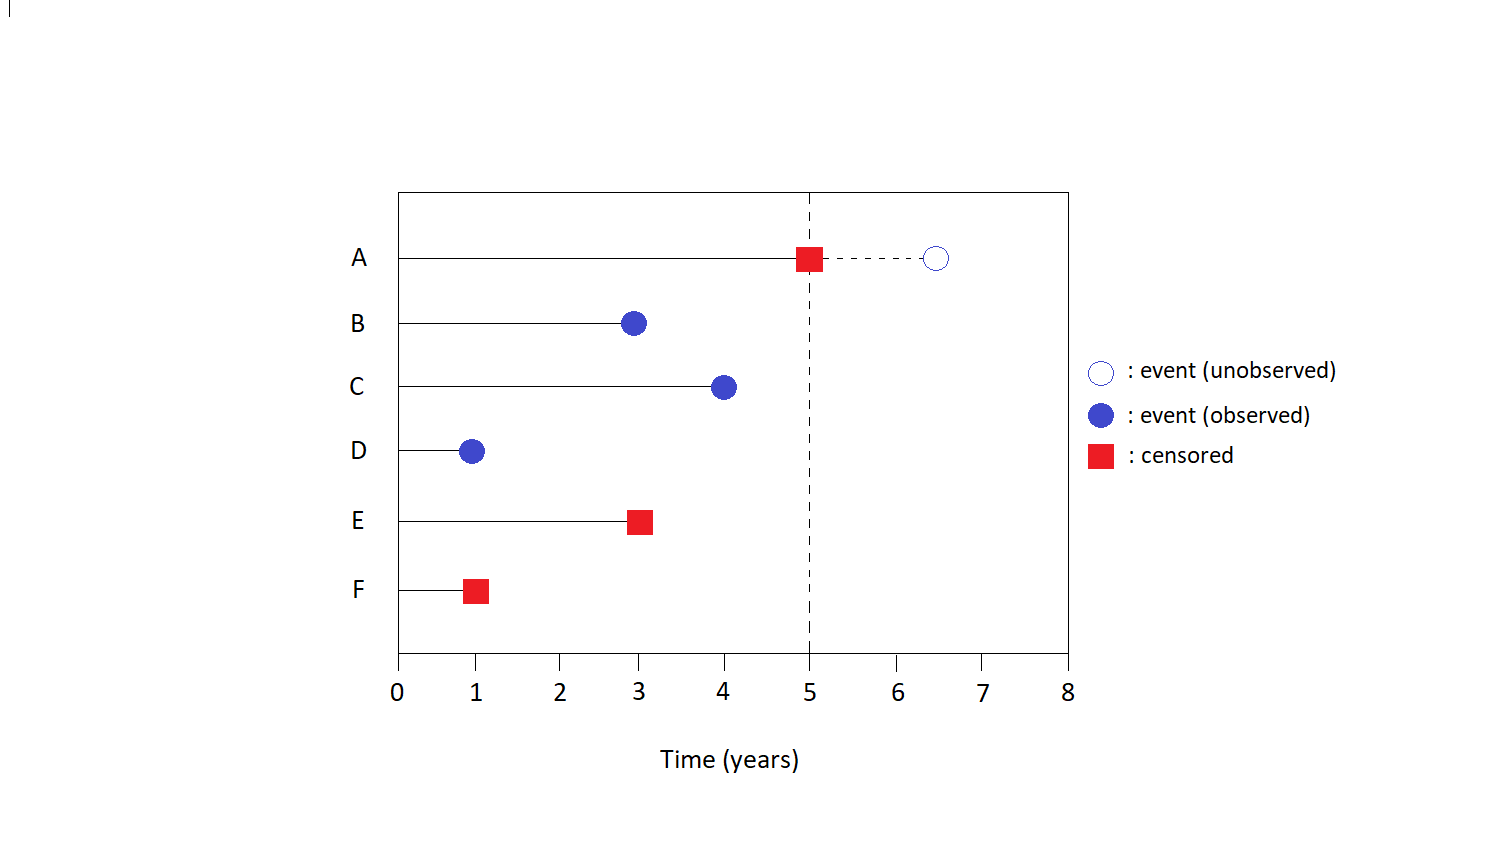
\includegraphics[width=1\linewidth]{figures/right_censoring_example} \caption{Right Censoring Example}\label{fig:rightcensoringexample}
\end{figure}

As illustrated by individual A in Figure
@ref(fig:rightcensoringexample), this individual lives on until the
termination of the study. We don't know at what point they passed away
exactly, since they didn't pass away during the time constraints of the
study. As such, the only information we have is \(T > 5\).

If an individual does pass away at some point, \(t_i\), \emph{during}
the study, then \(T = t_i\). This can be illustrated within Figure
@ref(fig:rightcensoringexample) by individuals B, C, and D for which
\(T = 3\), \(T = 4\), and \(T = 1\).

There is a final possibility for individuals who choose to censor
themselves. Illustrated in Figure @ref(fig:rightcensoringexample) by
individuals E and F, we can see that they are marked as censored at
\(T = 3\) and \(T = 1\), respectively. These individuals may have chosen
to stop submitting information to the study or drop out of the study
entirely without warning. As we have no information about whether or not
if they died or simply did not submit their form, all we know is that
the individual died/will die at some point after the point at which they
were censored.

Right censoring is the most common type of censoring and can often be
found in clinical trial studies, mortality studies, and other forms of
surival analyses.

\hypertarget{left}{%
\subsubsection{Left Censoring}\label{left}}

\begin{figure}
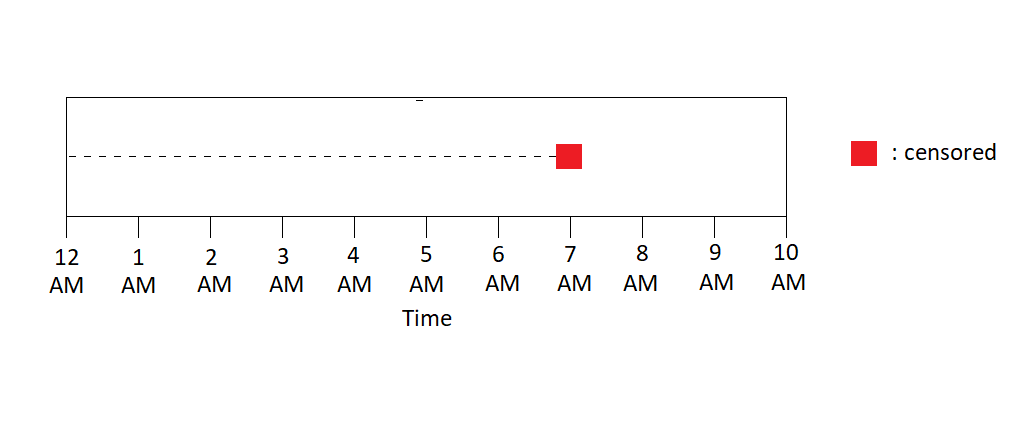
\includegraphics[width=1\linewidth]{figures/left_censoring_example_fix} \caption{Left Censoring Example}\label{fig:leftcensoringexample}
\end{figure}

In contrast with right censoring, left censoring is a specific instance
of censoring in which we only know that the true value of a data point
falls below a certain threshold which we call the \emph{limit of
detection} (LOD).

To understand this concept better, consider the following example.
Imagine a scenario in which you are attempting to estimate the time at
which the sun rises each morning. You plan to wake up every morning far
before the sun rises, but on the first day of the study, you oversleep
and wake up at 7:00 A.M. with the sun already out. We now have an
instance of left-censored data. We want to know the time at which the
sun rose, but all we have is an upper limit (7:00 A.M.).

Left censoring is commonly found in environmental, water quality, and
chemical-related research where the focus is on the concentration of an
analyte. Due to limitations on measuring instruments, left censored data
are commonly found in these types of studies. The most pressing issue of
left-censored data mostly lie in the difficulty of distinguishing
between extremely low values and statistical noise {[}@Hall2020{]}.

\hypertarget{interval}{%
\subsubsection{Interval Censoring}\label{interval}}

\begin{figure}
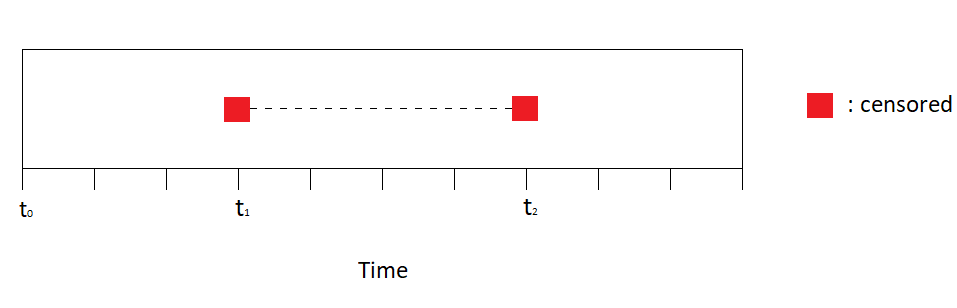
\includegraphics[width=1\linewidth]{figures/interval_censoring_example_fix} \caption{Interval Censoring Example}\label{fig:intervalcensoringexample}
\end{figure}

Interval censoring is another form of censoring in which the random
variable of interest is known to be between an interval of two values.
Considering a random variable \(T\), which denotes the survival time of
interest, if interval censoring is at hand, we can denote the interval
containing \(T\) to be \(I = [t_1, t_2]\), with \(t_1\) being the
beginning of the interval and \(t_2\) being the end of the interval.
Left and right censoring are special cases of interval censoring. In the
case of left censoring, \(t_1 = 0\); and conversely in the case of right
censoring, \(t_2 = \infty\).

To conceptualize interval censoring, we can consider a example study on
virus testing in which participants get their blood drawn in order to
detect whether or not they test positive for a virus or not. The random
variable in question is \(T\), which represents the exact timepoint at
which the subject contracted the virus. If an individual was first
tested at time \(t_1\) and tested negative, but was tested again at a
later time \(t_2\) and tested positive, the specific time \(t\) at which
the subject contracted the virus is unknown. All we know is that it lies
somewhere between the interval, \(I = [t_1, t_2]\), but not the exact
time at which they contracted it.

The focus of my thesis deals specifically with the challenges of
reporting and working with left-censored data.

\hypertarget{challenges}{%
\subsection{Challenges of Reporting Censored Data}\label{challenges}}

There is no universal reporting practice for values below the LOD which
can lead to confusion amongst researchers. The lack of standardization
makes it difficult to distinguish values below the LOD and uncensored
values. This can lead to values below the LOD unintentionally being
overlooked, causing faulty analysis or conclusions which are heavily
flawed.

In a study involving the precision of lead measurements near
concentrations of the limit of detection, @Berthouex1993 discusses the
disparity among chemists regarding practices involving the recording
values below the LOD. He enumerates the following list.

\begin{enumerate}
  \item Reporting the letters ND, "not detected"
  \item Reporting the numeric value of the LOD
  \item Reporting "< LOD", where LOD is the numeric value of the LOD 
  \item Reporting some value between 0 and the LOD, such as one-half the LOD
  \item Reporting the actual measured concentration, even if it falls below the LOD
  \item Reporting the actual measured concentration, followed by "(LOD)" 
  \item Reporting the actual measured concentration with a precision ($\pm$) statement
\end{enumerate}

According to @Gilbert1987, the latter three methods are the best
procedures to follow, especially from a practical and statistical point
of view. He argues that assuming the small concentration values are not
from some sort of measurement error during data collection, then the
measured concentration holds value. As such, recording a measurement as
``below LOD'' without any sort of accompanying value would be discarding
useful information which could have been used in practice and analysis.

@Berthouex1993 discusses the prevalence in regards to the practice of
censoring data by reporting only values which are above the detection
limit and discarding those which fail to yield quantifiable results. In
the study he conducted, five laboratories were assigned tasks to measure
samples of a certain solution. The laboratories were not given
information regarding the intent of the study, but a general statement
that the concentrations being measured were of ``low'' concentrations.
All but one laboratory recorded the actual measured concentrations even
though they fell below the LOD. Fortunately, the original measurements
for the laboratory that did not report values for all samples were
maintained and able to be recovered. @Berthouex1993 stresses the
importance of standardization in reporting practices for laboratories
and suggested reporting all measurements accompanied with some precision
statement, so that data is not lost.

Further supporting the stance of keeping all concentration measurements
rather than only those above the detection limit, Monte-Carlo
experiments were conducted by @Gillom1984 to investigate trend-detection
for water-quality data. Trend detection is the practice of determining
whether the values of a random variable generally increase or decrease
over a period of time. They found a general relationship of decreasing
trend detection percentages with increased censoring levels, attributing
this to the limited availability of information in censored data.

\hypertarget{Approaches}{%
\subsection{Parameter Estimation Techniques for Left-Censored
Data}\label{Approaches}}

It is important to note that the values below the LOD still contain
information, specifically that the values is between the lower bound
value (if it exists) and the LOD {[}@Chen2011{]}. As such, there are a
variety of statistical treatments to handle censored data which have
been popularized in the statistical literature.

Before we discuss the techniques which have been popularized through
literature and studies regarding parameter estimation with left-censored
data, it important to discuss \emph{omission}, the deletion of data
points which are deemed to be invalid as a result of left-censoring or
any other deficiencies in the data. As a result of being simple to
comprehend and implement, omission is a common technique used in lieu of
specialized techniques designed to handle missing data.

One type of omission is known as \emph{available-case analysis}, in
which statistical analysis is conducted while only considering the
observations which have no missing data on the variables of interest,
and excluding the observations with missing values {[}@May2012{]}. May
argues against this approach and claims that the loss of information
from discarding data and the inflation of standard errors of estimates
(when discussing missingness in a regression context) will invariably be
inflated as a result of the decreased sample size.

Over the past century, a myriad of methods to deal with censoring have
been developed to counter this issue of discarding data with
omission-based techniques -- some more statistically sound than others.
We will review some of the more common methods to estimate descriptive
statistics involving censored data, which include: substitution, maximum
likelihood estimation, Kaplan-Meier, and regression on order statistics.

\hypertarget{Substitution}{%
\subsubsection{Substitution Method}\label{Substitution}}

The first technique we will discuss is the substitution method, which
involves imputing in a replacement value in lieu of the censored data
point. As a method commonly condemned in papers as a statistically
unsound method to handle censored data, substitution methods are
ubiquitous in the chemical and environmental sciences
{[}@Canales2018{]}.

Substitution techniques are easy to understand and to implement, akin to
the omission techniques we discussed previously. Observations for which
measurements fall below the LOD are replaced with a replacement value,
which is non-specific and can vary between studies. A non-exhaustive
list of common replacement values include:
\(\frac{LOD}{2}, \frac{LOD}{\sqrt2}\), and the \(LOD\) itself
{[}@Lee2005{]}.

Proponents of the substitution method claim that the replacement value
\(\frac{LOD}{2}\) is useful for data sets in which the majority of the
data are below the LOD or when the distribution of the data is highly
skewed; the definition of ``highly skewed'' being any distribution with
a geometric standard deviation (a measure of spread commonly used in
tandem with log-normal distributions) of 3 or more {[}@Hornung1989{]}.
They also suggest using \(\frac{LOD}{\sqrt2}\) when there are only a few
data points below the LOD or when the data is not highly skewed.

Regardless of which replacement value is used, once a dataset is
generated containing these replacement values, analysis continues as is,
utilizing this new dataset.

As mentioned previously, contention between whether this method is
statistically sound or not remains to the present day. The lack of a
global, standardized replacement value to substitute is one of the most
pronounced downsides of this method. Different disciplines have their
own suggested ``best'' replacement value to use, an example being
\(\frac{3}{4}\) times the LOD being a common replacement value in
geochemistry {[}@Crovelli1993{]}. Due to the lack of standardization,
many regard substitution techniques as a non-rigorous, statistically
unsound method for handling left-censored data {[}@Chen2011{]}.

@Lee2005 also provides a critique on substitution methods and claim that
they can often introduce a ``signal'' which was not originally present
within the data, or even obstruct an actual signal which was originally
present in the data -- leading to misleading and/or inaccurate results.
Supporting @Lee2005's claim, Glass and Gray (2001) found the
substitution method to introduce large errors and biases when
calculating descriptive statistics of interest with left-censored data.
Thompson and Nelson (2001) conducted a study in which they found similar
results, in that it often led to biased parameter estimates and
``artificially small standard error estimates.'' Hewett and Ganser
(2007) also found in their simulation study that the substitution method
yielded the lowest average bias and root mean squared error values
(comparison metrics to measure accuracy) in their estimation of the
mean. Overall, the overall consensus seems to advise against the
practice of these substitution techniques.

\hypertarget{MLE}{%
\subsubsection{Maximum Likelihood Estimation}\label{MLE}}

Maximum likelihood (ML) estimation is a parametric technique which
allows us to estimate the parameters of a model when the data are from a
known distribution.

Let the random variables \(X_i, \cdots, X_n\) be independent and
identically distributed with probability function \(f(x_i|\theta)\),
where \(\theta\) is the parameter we are interested in estimating.

For every observed random sample \(x_1,\cdots,x_n\), the joint density
function is:

\[f(x_1,...,x_n|\theta) = f(x_1|\theta)...f(x_n|\theta) = \prod_{i=1}^{n}f(x_i|\theta)\]

Our goal is to find the value of \(\theta\) which is most likely to
generate our observed data. In order to solve this inverse problem, we
introduce the likelihood function, which is defined as a function of the
parameter given the observed data:

\[L(\theta) = L(\theta|x_i, \cdots, x_n) = \prod_{i=1}^{n}f(x_i|\theta)\]
Our \emph{maximum likelihood estimate} of our parameter \(\theta\),
then, is the value \(\hat{\theta}\) that maximizes the likelihood
function, \(L(\theta)\).

When left censoring is present, the likelihood function changes in order
to account for both the censored observations and the uncensored
observations. We define \(F(x_i|\theta)\) to the cumulative distribution
function for our RVs conditioned on \(\theta\). Our new likelihood
function when left censoring is present is:

\[lik(\theta) = \prod_{i=1}^n f(x_i|\theta)^{\delta_{i}} \ \times F(x_i|\theta)^{1-{\delta_{i}}}\]

\noindent where \(\delta_{i}\) indicates whether or not the \(i\)th
observation is censored:

\[\delta_i =
\begin{cases}
  0 & \text{if censored} \\
  1 & \text{if uncensored}
\end{cases}\]

It is then possible to follow typical procedures to find the maximum
likelihood estimates of the parameteres of interest (mean, variance,
etc.) from our censored data.

@Yavuz2017 discusses the usage of ML estimation when missing data is
present, and notes it is only appropriate for non-negative probability
distributions such as the exponential, log-normal, and Weibull models.
This is one limitation of ML estimation, it cannot be applied for data
which do not fit a specified model -- and is very limited in scope.

ML estimation is one of the most well-known parametric approaches to
handling left-censored data. Many studies use ML estimation as a
baseline method of handling censored values, to which they compare their
new techniques {[}@Ganser2010{]}. Despite its prevalence, ML estimation
has its weaknesses. @Canales2018 found that the ML estimation seems to
underperform when the data in question was highly skewed, producing
overinflated mean squared errors. Additionally, because ML estimation is
so heavily dependent upon distributional assumptions, an incorrect
specification of the distribution of the censored data will inevitably
lead to misleading results {[}@Bolks2014{]}. Regardless of these
limitations, it is a definite staple in the field of parameter
estimation with regards to censored data.

\hypertarget{rkm}{%
\subsubsection{Kaplan-Meier Method}\label{rkm}}

As a phenomenon, censoring is most often discussed in survival analysis,
which concerns itself with techniques to analyze a \emph{time to an
event} variable. As its name suggests, these variables measure the time
which passes until some event of interest occurs. This can be as
innocuous as the time until a device breaks, time until birds migrate
away from their homes, time until a person passes away, etc. In all
cases, there is a possibility of the data being censored.

The Kaplan-Meier (KM) method is a common nonparametric technique used to
deal with censored data. Nonparametric methods do not make assumptions
about the underlying distribution of the data. The KM method was
originally developed to handle right-censored survival analysis data
{[}@Hall2020{]}. The advantages of the KM method lies in its robustness
as a nonparametric method -- it performs well without having to depend
upon distributional assumptions. Many recommend its usage in cases of
severe censoring, instances where more than 90\% of the data is censored
{[}@Canales2018{]}.

The KM-estimator is a statistic used to estimate the survival curve from
the data while accounting for censoring. It does this by assuming that
censoring is independent from the event of interest and that survival
probabilities remain the same in observations found early in the study
and those recruited later in the study {[}@Gillespie2010{]}.

The KM-estimator of the survival curve at time \(t\) is:

\[\hat{S}(t) = \prod_{\ t_i \le \ t }\left(1-\frac{d_i}{n_i}\right)\]

where \(t_i\) is the distinct event time, \(d_i\) is the number of event
occurrences at time \(t_i\), and \(n_i\) is the number of followup times
(\(t_i\)) that are greater than or equal to \(t_i\) (how many
observations in sample survived until at least time \(t_i\))
{[}@Klein2003{]}.

Typically, the KM-estimator is used to estimate the distribution
function of right-censored data. Helsel (2005, as cited in Yavuz et al.,
2017) provided a simple modification of the KM-estimator to allow for
the estimation of the survival curve with left-censored values. In his
implementation, he ran the left-censored data through a transformation
algorithm before using the KM method to change them into right-censored
data.

The transformation algorithm works as follows: First, all the
left-censored values in the dataset are arranged in descending order of
magnitude. Then these left-censored values are subtracted from \(M\), to
get \(M-x_i\), the newly transformed, right-censored value (\(M\) is a
constant bigger than the maximum value in the dataset). Finally, the
non-censored values and the newly transformed values are then arranged
in ascending order to be used to estimate the survival function through
the Kaplan-Meier estimator.

The KM-method is not an imputation procedure, but instead an estimation
technique that allows for the calculation of descriptive statistics for
left-censored datasets. @She1997 gives the expressions to calculate the
estimated mean, median, and variance:

\begin{table}[h]
\begin{tabular}{ll}
\textbf{Descriptive Statistic} & \textbf{Expression}                                                                                              \\
Mean ($\hat{\mu}$)             & $\hat{\mu} = \displaystyle \int_{0}^{\infty} \hat{S}(t) \ dt$                                                    \\
Median ($\hat{M}$)             & $\hat{M} = \displaystyle \hat{S}^{-1} \left (\frac{1}{2} \right)$                                                              \\
Variance ($Var(\hat{\mu}$)     & $Var(\hat{\mu}) = \displaystyle \sum_{i=1}^{r} \left( \int_{t_i}^{\infty}\hat{S}(t) \ dt \right)^2 \frac{d_i}{n_i(n_i - d_i)}$
\end{tabular}
\end{table}

\hypertarget{ROS}{%
\subsubsection{Regression on Order Statistics}\label{ROS}}

Lastly, regression on order statistics (ROS) combines both the
parametric nature of the MLE approach and nonparametric nature of the KM
method. ROS is a semi-parametric method which assumes an underlying
distribution (usually lognormal) for the censored measurements but makes
no assumption towards the distribution of uncensored measurements.

@EPA2009 provides a a more detailed explanation to the methodology of
ROS, but the basic procedures will be outlined in this thesis.

A brief explanation as to how ROS works is as follows. ROS begins with
the estimation of the cumulative probability associated with each
distinct LOD. This cumulative probability is distributed equally between
the censored values with a common LOD. Once the censored values are
ranked, a linear regression model is fit between the uncensored values
and the distributional z-scores from the censored probability plot. The
parameters of the regression model (slope and intercept of the
regression line) is then used to estimate the mean and standard
deviation of the distributional model which are then used to generate
imputed values for the censored observations.

Delving into the mathematics behind this procedure, we need to first
define several variables.

We define \(k\) be the number of distinct LODs in the data, \(A_i\) as
the number of uncensored values between the \(i\)th and \((i+1)\)th LOD
for \(i=1\) to \(k-1\), and \(A_k\) as the number of uncensored values
above the highest LOD, \(A_0\) as the number of uncensored values below
the lowest LOD.

We also define \(B_i\) as the total number of observations (both
uncensored and censored) with values below the \(i\)th LOD and
\(B_0 = 0\).

\begin{equation}
$e = mc^2$
\end{equation}

In order for ROS to be utilized, there needs to be at least 5 known
values and more than half the values within the censored variables must
be known. As regression is utilized in this method, the response
variable must also be a linear function of the explanatory variable
(quantiles). Additionally, the errors should have constant variance
{[}@Lee2005{]}.

The \texttt{NADA} package contains the function \texttt{ros} which
provides an implementation of regression on order statistics which
allows us to calculate descriptive statistics for left censored values.

{[}INSERT PARAGRAPH TO TRANSITION TO CHAPTER 3 (?){]}

\end{document}
